\label{sec:NuMUCCsel}

\par This selection is designed to be best used as a constraining tool for the $\nu_e$ analysis. The flux and cross-section predictions for BNB $\nu$s are most uncertain in the few-hundreds MeV energy region, blurring the results of a low-energy analysis focused on that region of phase space. Because the $\nu_e$s and $\nu_{\mu}$s share the same parent hadronds and interact similarly in the detector, the $\nu_{\mu}$ sample can be used to constrain flux and cross-section uncertainties in the intrinsic $\nu_e$ rate expectation. Furthermore, the $\nu_{e}$ selection is subject to higher uncertainties due to its low statistics, but the $\nu_{\mu}$ channel benefits from two orders-of-magnitude larger absolute flux.

\par This selection is ultimately a $\nu_{\mu}$ CC Inclusive selection, allowing any number of final state hadrons, with a focus on prioritizing performance in the low-energy region. This selection is intentionally broad, this accomplishes a few things. It allows for the quick implementation of exclusive sub-selections that can probe interesting features in the data, and also provides ample the statistics. The selection described here employs only on Run3 data in order to rely on the CRT for additional cosmic rejection, as will be described later. %The improved statistics are important because only Run 3 is considered in this selection, this will be discussed later in the section. 

\par \cref{ssec:NuMUCCsel:sel:vars} defines the variables used in this selection. \cref{sssec:NuMUCCsel:constr:selectionandsignal} further defines the signal and the cuts placed on the variables described in \cref{ssec:NuMUCCsel:sel:vars}. \cref{ssec:NuMUCCsel:datasample} discusses the data sample used for the constraint. And \cref{ssec:NuMUCCsel:timedep} discusses the time dependence of the data.

%-----------------VARIABLE DEFINITIONS---------------------%
\subsection{Variable Definitions}
\label{ssec:NuMUCCsel:sel:vars}

\par Table~\ref{tab:numuvariableSummary} contains a concise list of variables used in this $\nu_{\mu}$ selection. The variables are organized into \textit{event} and \textit{track}-level descriptors, used for preselection and muon-candidate selection respectively. There is some redundancy between this list and the list in sec \ref{sec:nueselection:variables}, but this list below should serve as a quick reference to a reader of this chapter.

\begin{table}[H]
\caption{\label{tab:numuvariableSummary} Summary of the definition for the variables used in the $\nu_{\mu}$ selections.}
\centering
\begin{tabular}{ m{0.07\textwidth} | m{0.26\textwidth} | m{0.55\textwidth}  }
Category & Variable Name & Description  \\
\hline

\multicolumn{1}{l|}{} & \texttt{nslice} &  Number of neutrino slices identified by the \texttt{SliceID}. Values are  0 or 1.\\  \cline{2-3}
\multicolumn{1}{l|}{} & \texttt{crtveto} & Boolean variable checking if the event passes the CRT veto. Not available for Run 1 and Run 2 data. \\  \cline{2-3}
\multicolumn{1}{l|}{} & \texttt{reco\_nu\_vtx\_sce\_\{x,y,z\}} & Reconstructed neutrino interaction vertex in (x,y,z) coordinates. The space charged correction is applied.  \\  \cline{2-3}
\multicolumn{1}{l|}{} & \texttt{n\_tracks\_contained} &  number of tracks fully contained in the fiducial volume.\\  \cline{2-3}
\multicolumn{1}{l|}{} & \texttt{slpdg} &  PDG code of the event as assigned by Pandora, 12 if the object with the most hits over all planes is shower-like, 14 if track-like.\\  \cline{2-3}
%\multicolumn{1}{l|}{} & \texttt{all\_\{start,end\}\_contained} &  The start/end points of all PFParticles are volume defined with borders: \SI{5}{\cm} in $x$ and \SI{6}{\cm} $y$ and \SI{10}{\cm} $z$.\\  \cline{2-3}
\parbox[t]{2mm}{\multirow{4}{*}{\rotatebox[origin=c]{90}{Slice}}} & \texttt{hits\_ratio} & Ratio between hits from showers and total number of hits in the slice. \\  \cline{2-3}
\multicolumn{1}{l|}{} & \texttt{CosmicIP} & Closest distance between shower start and space points associated to tracks flagged as cosmics. \\  \cline{2-3}
\multicolumn{1}{l|}{} & \texttt{\_closestNuCosmicDist} &  3D distance between the reconstructed neutrino vertex and the closest CRT-tagged cosmic track. \\  \cline{2-3}
\hline

\multicolumn{1}{l|}{} & \texttt{trk\_sce\_\{start,end\}\_\{x,y,z\}} &  Reconstructed, spacecharge-corrected start/end-points for the tracks.\\  \cline{2-3}
\multicolumn{1}{l|}{} & \texttt{trk\_llr\_pid\_score} &  The log likelihood ratio particle identification score (see sec. \ref{subsec:loglikelihoodpid}). This variable has strong muon-proton discriminating power (see fig. \ref{fig:llr_pid_uvy_example}).\\  \cline{2-3}
\multicolumn{1}{l|}{} & \texttt{trk\_score} & A machine-learned quantity that describes how `track-like' the reconstructed object is (possible values between 0 and 1). \\  \cline{2-3}
\parbox[t]{2mm}{\multirow{4}{*}{\rotatebox[origin=c]{90}{Track}}} & \texttt{trk\_len} & The length of the reconstructed track (in cm). \\  \cline{2-3}
\multicolumn{1}{l|}{} & \texttt{trk\_distance} & The distance from the start-point of the reconstructed track to the reconstructed neutrino vertex (in cm). \\  \cline{2-3}
\multicolumn{1}{l|}{} & \texttt{pfp\_generation} &  The generation of the PFParticle according to Pandora: the neutrino has generation 1, its direct daughters 2, and further decay products 3 or higher.\\  \cline{2-3}
\multicolumn{1}{l|}{} & \texttt{MCS\_quality} &  Agreement between the muon momentum estimated with the range-based method $P_\texttt{range}$ and with the Multiple Coulomb Scattering-based method $P_\texttt{MCS}$. The variable is defined as $(P_\texttt{MCS}-P_\texttt{range})/P_\texttt{range}$.\\  \cline{2-3}
\hline

\end{tabular}
\label{tab:numuvariableSummary}
\end{table}

\subsection{Selection}
\label{sssec:NuMUCCsel:constr:selectionandsignal}

\par A $\nu_{\mu}$ event is identified by the presence of one muon candidate originating from inside the fiducial volume of the TPC. Additional tracks may accompany the muon candidate; additional particles assist in the neutrino event reconstruction and energy calculation but their information is not used in the selection itself. Showers are not explicitly rejected although they contribute very little to the final spectra, particularly in the low-energy region. 

\par This selection filter can be broken down into ``preselection'' and ``muon selection'' components. The preselection filter is applied first and only takes event-level variables as input. In other words, the preselection filter is coarse and interacts only with variables that reflect the event as a whole but are agnostic to features of individual tracks. The primary purpose of the preselection is to eliminate events that are founded on cosmic muons or are not generally $\nu_{\mu} CC-like$. The events that pass through the preselection filter are then put through the muon selection filter. If the event does not have at least one track that passes the requirements than it is rejected. If multiple tracks pass the filter, the longest one is selected as the muon candidate. 

\par Many supporting plots for this section are in \cref{sec:Appendix:numu:constr}, where one can find the distributions of every variable cut on in the selection. 

\subsubsection{Event Preselection}
\label{sssec:NuMUCCsel:constr:preselec}

\par The $\nu_{\mu}$ constraint selection is built from the groundwork of the SliceID tool (sec. \ref{sec:sliceID}) like the $\nu_e$ selections of this analysis are; SliceID selects $\nu-like$ events and is agnostic to flavor. The additional preselection cuts are chosen to reduce cosmic and dirt backgrounds and select slices that are generally more $\nu_{\mu}$-like. 

\par \cref{tab:numuCC:presel} summarizes the preselection cuts. 
The containment requirement on the reconstructed vertex favors $\nu_{\mu}$ CC events and disfavors cosmogenic or dirt-like activity as the latter originate from outside the detector. The topological score is a machine learned quantity that is designed to discriminate between events founded on muons from cosmic vs neutrino parents. The final cut on the $z$ coordinate is to avoid a region of the MicroBooNE detector with non-functioning channels~\cite{bib:noise} -- a common practice within the collaboration. \\

\par Three variables of the preselection are informed by the cosmic ray tagger (CRT) system at MicroBooNE, $CRT\ Veto$, $crthitpe$, and $closestNuCosmicDist$. The first two reflect whether or not the CRT system was triggered in coincidence with the event and how many photoelectrons (PEs) were recorded by the CRT system. One can further extrapolate straight lines between a CRT hit and reconstructed track end-points, allowing for additional CRT+topology rejection. The distance between that extrapolated CRT-tagged track and the reconstructed neutrino vertex is given in the third variable, $closestNuCosmicDist$. The CRT cuts remove a significant amount of the off-beam data, particularly at lower reconstructed energies. The effect of the CRT cuts on this selection can bee seen in the Appendix, Fig \ref{fig:NuMuCCsel:crtimpact}.

\par Finally, it is required that 90$\%$ of all hits in the reconstructed slice are contained inside the fiducial volume, via $contained\_fraction$.

\par Ensuring that all events are contained is a crux of this selection, it is consistent with the stated goal of constructing a selection that prioritizes low-energy performance. Muons from low-energy $\nu_{\mu}$s will not have much kinetic energy and often decay inside the nearly ten meter long detector. Nearly all muons that trigger the CRT system will be cosmogenic, from a high-energy $\nu_{\mu}$, or a $\nu_{\mu}$ close to the edge of the detector. Range-based energy reconstruction (using the Bethe-Bloch formula) can be done on contained tracks, but not un-contained ones, where multiple coulomb scattering (MCS)-based measurements can be done on any track that is at least 50 cm long but provides a less precise measurement. The range-based energy calculations are used in the final $\nu_{\mu}$ energy calculation, but the MCS-based calculations are used for validation, more on this later. 

\begin{table}[h!]
\centering
\setlength{\tabcolsep}{10pt}
\renewcommand{\arraystretch}{1.25}
 \begin{tabular}{| c | c |} 
 \hline
 Cut goal & Cut definition \\
 \hline\hline
 \multirow{1}{*}{ Cosmic rejection } & nslice = 1 \\
 \hline
 \multirow{4}{*}{Fiducial Volume} & \texttt{reco\_nu\_vtx\_sce\_x} $\in$ [5,251] cm \\ &
\texttt{reco\_nu\_vtx\_sce\_y} $\in$ [-110,110] cm \\ &
\texttt{reco\_nu\_vtx\_sce\_z} $\in$ [20,986] cm \\ &
\texttt{reco\_nu\_vtx\_sce\_z} $\not\in$ [675,775] cm.\\
\hline
\multirow{1}{*}{Signal~topology} & \texttt{topological\_score} $>$ 0.06 \\
 \hline
 \multirow{2}{*}{ Cosmic rejection (Run3) } & \texttt{CRT Veto} != 1 or \texttt{crthitpe} $<$ 100\\
& \texttt{closestNuCosmicDist} $>$ 5 cm\\
 \hline
Containment & \texttt{contained\_fraction} $>$ 0.9 \\
 \hline
 \end{tabular}
 \caption{\label{tab:numuCC:presel} Preselection requirements for the $\nu_\mu$ constraining selection.}
\end{table}


\subsubsection{Muon Selection}
\label{sssec:NuMUCCsel:constr:muonsel}

\par After the event-level cuts are applied, the tracks in the slice are further analyzed to identify individual muon candidates. At least one reconstructed track in the event must satisfy all the criteria listed in table \ref{tab:findthemuon} for the event to pass the selection. If more than one track passes this requirement, then the longest is taken as the muon candidate. Of the muon candidates that pass this selection, $\approx 94\%$ are, in simulation, correctly tagged muons from $\nu_{\mu}$ CC interactions.

\par The cuts made on the start and end points of the reconstructed tracks require that the track is fully contained inside the fiducial volume of the detector. The preselection requires that the vertex and most of the hits be contained, but not all the tracks themselves. This containment cut further eliminates cosmic muons enables the use of range-based energy calculations for the muon. The final `cosmic rejection' cut is the requirement that the reconstructed muon start point is no more than four cm from the reconstructed neutrino vertex. This eliminates events that are just cosmic muons that happen to be somewhat close to some hadronic activity. 

\par The log-likelihood variable, see \cref{subsec:loglikelihoodpid}, is a powerful muon-proton discriminator, with values close to -1 being proton-like and values close to +1 being muon-like. The cut at 0.2 avoids the ambiguous region close to 0 dominated by cosmic events and more susceptible to detector uncertainties. Additionally, the track is required to be at least 10 cm long to be muon-like.

\par The track score cut ensures that the selected tracks are particularly track-like and this removes many track-like showers from the selection.  The PFParticle generation cut ensures that Pandora recognizes that the track is produced directly at the neutrino interaction vertex, and not as a secondary particle (i.e. in a $\pi \rightarrow \mu$ decay or re-interaction). 

\par A final selection cut requiring agreement between the muon's range-based and MCS-based momentum is imposed. This cut provides an additional handle to increase purity and the quality of the reconstruction of $\nu_{\mu}$ events (see figs \ref{fig:NuMUCCsel:ryan:MCSqualitydistrib} and \ref{fig:NuMUCCsel:ryan:MCSqualityeres}). A `broken track' in the detector would fail this momentum quality test, for example. 

\begin{table}[h!]
\centering
\setlength{\tabcolsep}{10pt}
\renewcommand{\arraystretch}{1.25}
 \begin{tabular}{| c | c |} 
 \hline
 Cut goal & Cut definition \\
 \hline\hline
\multirow{6}{*}{ Containment } &
     \texttt{trk\_sce\_start\_x} $\in$ [5,251] cm. \\&
     \texttt{trk\_sce\_start\_y} $\in$ [-110,110] cm.\\&
     \texttt{trk\_sce\_start\_z} $\in$ [20,986] cm.\\&
     \texttt{trk\_sce\_end\_x} $\in$ [5,251] cm.\\&
     \texttt{trk\_sce\_end\_y} $\in$ [-110,110] cm.\\&
     \texttt{trk\_sce\_end\_z} $\in$ [20,986] cm.\\
   \hline
 \multirow{1}{*}{ Cosmic Rejection } & \texttt{trk\_distance} $<$ 4 cm.\\
 \hline
 \multirow{2}{*}{ Track Id } &
     \texttt{trk\_llr\_pid\_score} $>$ 0.2.\\&
     \texttt{trk\_length} $>$ 10 cm.\\
     \texttt{trk\_score} $>$ 0.8.\\ 
     \hline
 \multirow{1}{*}{ Direct $\nu$ Daughter } &     
                    \texttt{pfp\_generation} = 2.\\
  \hline          
 \multirow{1}{*}{ Reconstruction Quality } & -0.5 $<$ \texttt{MCS\_quality} $<$ 0.5\\
  \hline
\end{tabular}
 \caption{\label{tab:findthemuon} Requirements for $\mu$ identification.}
\end{table}

\begin{figure}[hbt!] 
\begin{center}
    \begin{subfigure}[b]{0.45\textwidth}
    \centering
    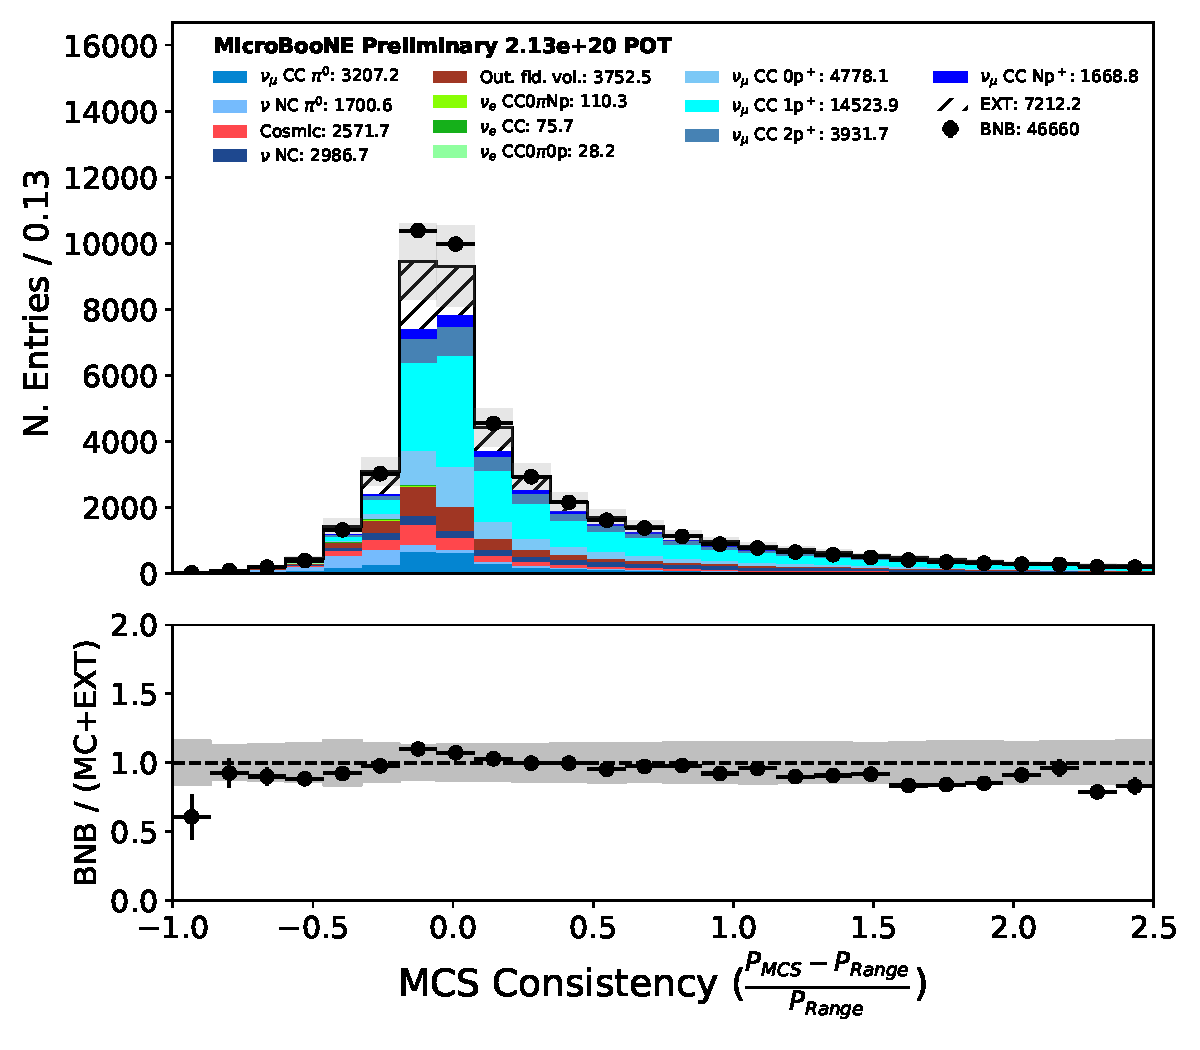
\includegraphics[height=5cm]{NuMuCCsel/Images/Ryan/appendix_muonsel_input_R3/trk_p_quality_v_07232020_presel_samples_detsys_event_category.pdf}
    \caption{\label{fig:NuMUCCsel:ryan:MCSqualitydistrib} Momentum quality variable distribution.}
    \end{subfigure}
    \begin{subfigure}[b]{0.45\textwidth}
    \centering
    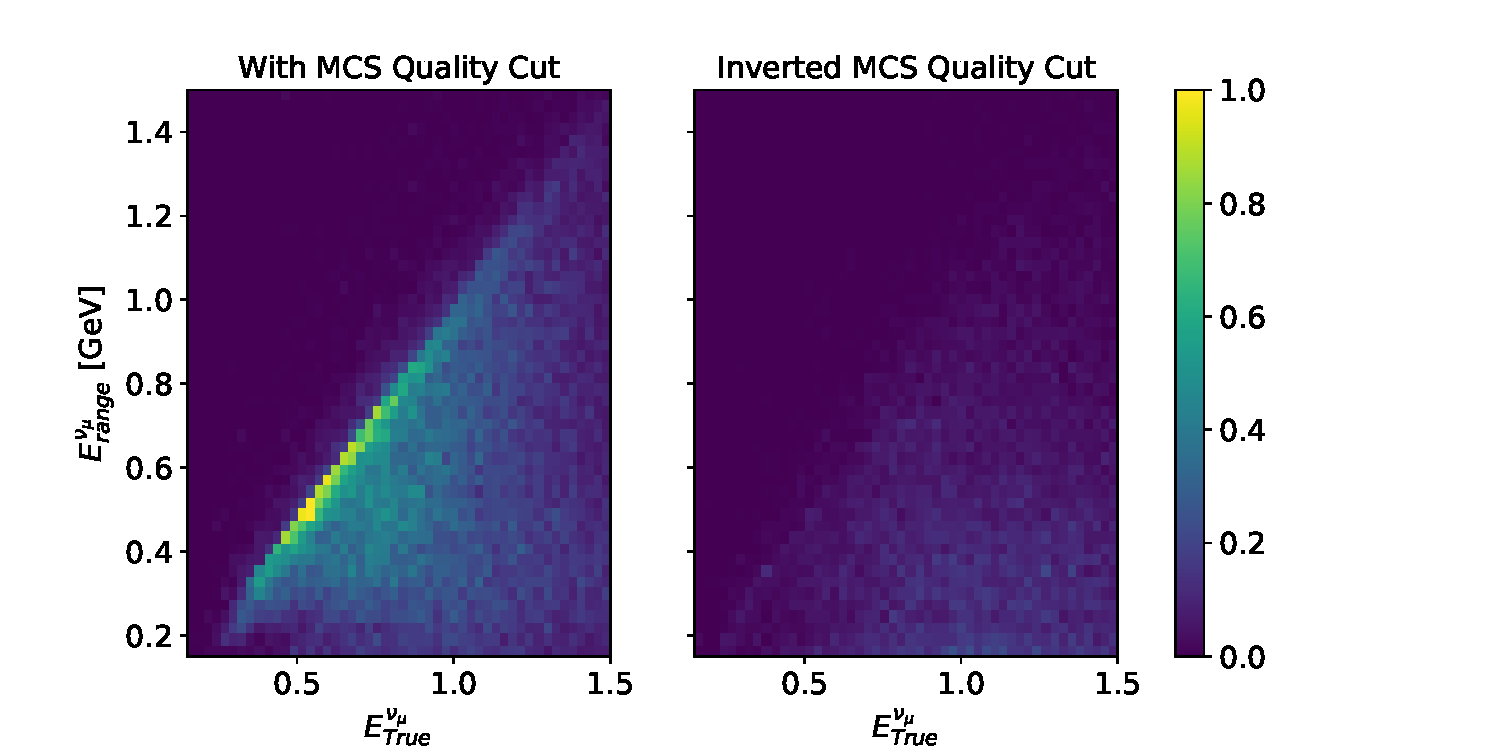
\includegraphics[height=5cm]{NuMuCCsel/Images/Ryan/other/EnergyRes_03202020_subplots.pdf}
    \caption{\label{fig:NuMUCCsel:ryan:MCSqualityeres} Events kept and rejected by the MCS cut.}
    \end{subfigure} \newline
\caption{MCS quality cut on preselected events.}
\label{fig:numusel:momres}
\end{center}
\end{figure}

\subsection{Data Sample}
\label{ssec:NuMUCCsel:datasample}

\par Run 3 is the only run used in the $\nu_{\mu}$ constraint, despite Run 1, Run 2, and Run 3 all being currently available and are presented in other sections of this note. The primary motivation for this decision is that the CRT variables (\cref{sec:sliceID:CRT}) are available only for Run 3. It was described in the previous section that the CRT cuts a crucial component of the selection. Given that this measurement on Run3 alone is not statistics limited, it was decided that the purity which can be achieved with the CRT cuts is more important than the higher statistics of all three runs. 

\par The inclusion of the CRT cuts, see \cref{tab:numuCC:presel}, removes nearly 64$\%$ of comic muon background, the primary background for $\nu_{\mu}$ CC events. Muons are particularly hard to reject at low energies without the CRT cuts; this is precisely where we want the highest purity. The uncertainty due to to cross-section and flux modeling is very high at low-energies for the $\nu_e$ analysis, boosting the importance of a pure $\nu_{\mu}$ sample in that region. One can see from the figures in appendix~\ref{sec:Appendix:numu:constr} that the CRT cuts does not degrade the DATA-MC agreement.

\subsection{Performance}
\label{sssec:NuMUCCsel:performance}
                    
\par Figure~\ref{fig:NuMuCCsel:run3kinematics} shows the reconstructed muon energy, muon angle, and neutrino energy with the available Run3 open data. With current open Run3 POT, we see $\mathcal{O}$($10^3$) entries per bin, making obtaining a constraint for flux and cross-section systematics with Run3 alone not a limitation to the analysis. Figure~\ref{fig:NuMuCCsel:ryan:runscombinedkinematics} shows the same distributions with the open data from all three runs, where more than three times the statistics are available. Plots from Runs other than Run 3 do not include the CRT cuts. It is worth pointing out that comparisons between Run3 and data from all three runs show consistent features, giving confidence in the analysis choice to rely on Run3 data for the constraint. This topic is further explored in the next subsection.

%-------RUN 3-----------
\begin{figure}[hbt!] 
\begin{center}
    \begin{subfigure}[b]{0.3\textwidth}
    \centering
    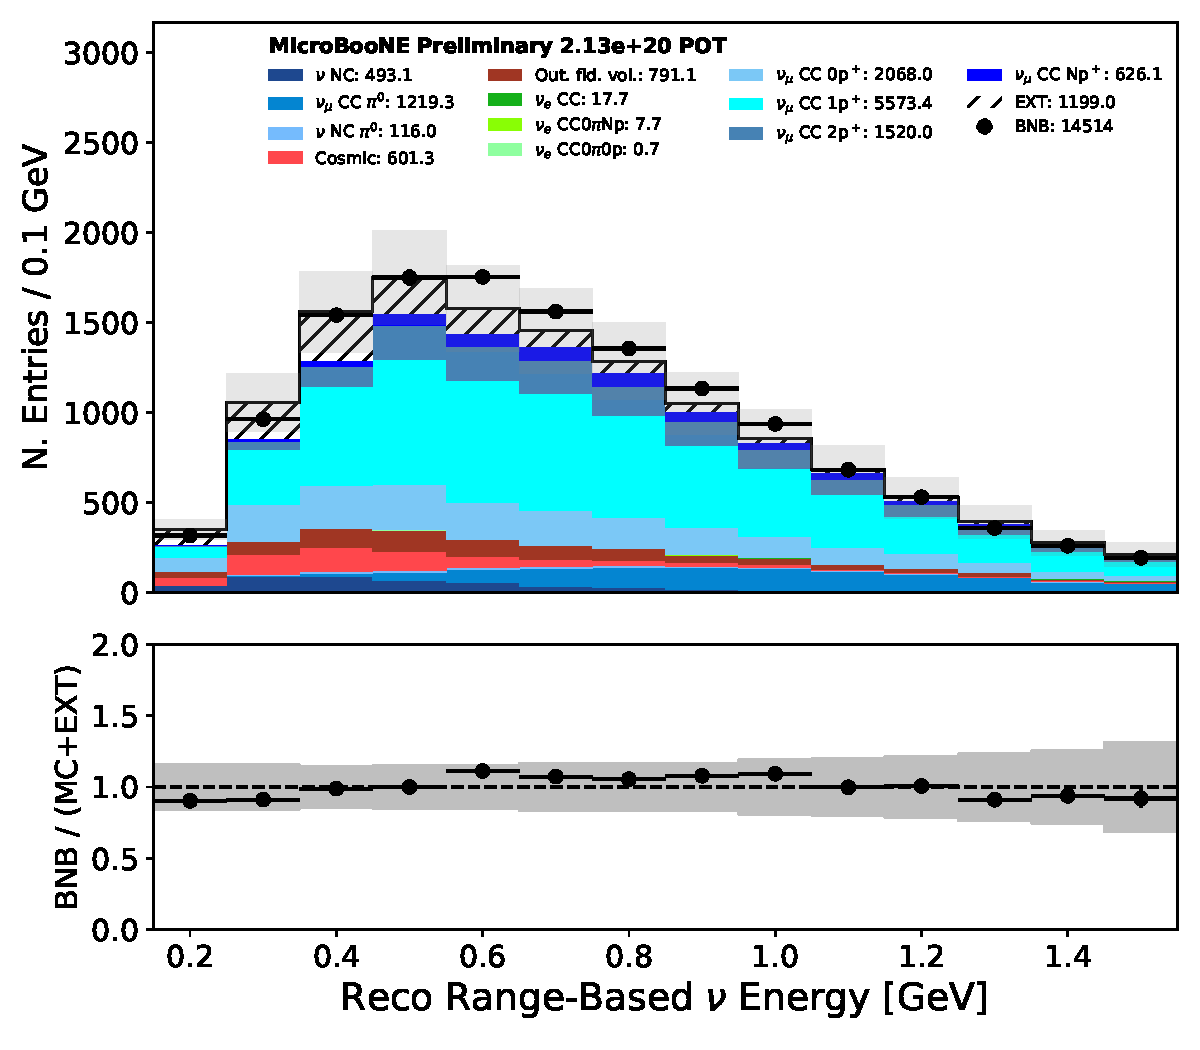
\includegraphics[width=1.00\textwidth]{NuMuCCsel/Images/Ryan/fullselection_run3_fullsystematics/reco_nu_e_range_v_07232020_fullsel_samples_detsys_event_category.pdf}
    \caption{\label{fig:NuMUCCsel:ryan:run3kinematics:nuE}}
    \end{subfigure}
    \begin{subfigure}[b]{0.3\textwidth}
    \centering
    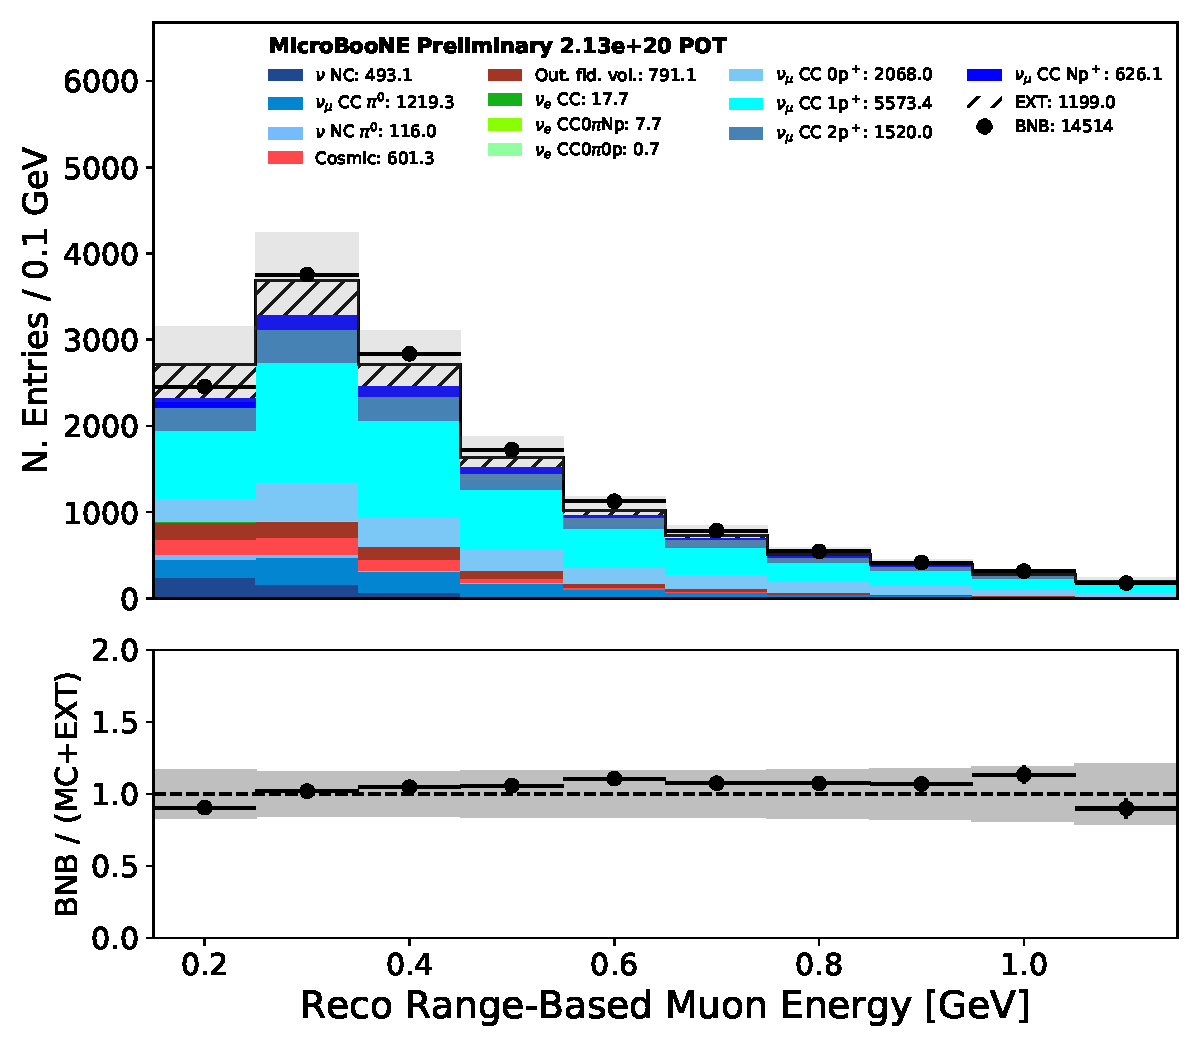
\includegraphics[width=1.00\textwidth]{NuMuCCsel/Images/Ryan/fullselection_run3_fullsystematics/trk_range_muon_e_v_07232020_fullsel_samples_detsys_event_category.pdf}
    \caption{\label{fig:NuMUCCsel:ryan:run3kinematics:muonE}}
    \end{subfigure}
    \begin{subfigure}[b]{0.3\textwidth}
    \centering
    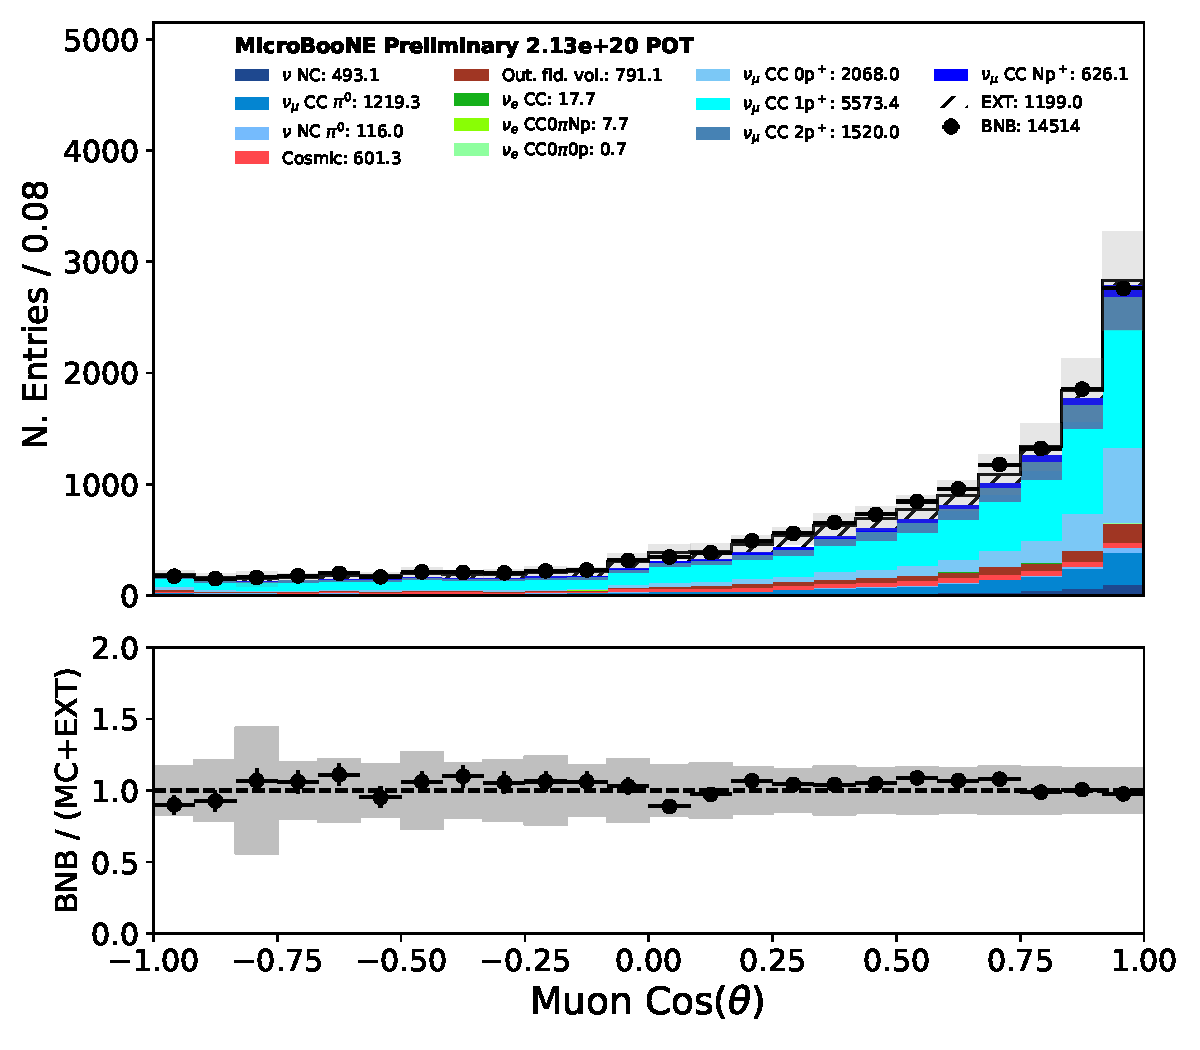
\includegraphics[width=1.00\textwidth]{NuMuCCsel/Images/Ryan/fullselection_run3_fullsystematics/trk_cos_theta_v_07232020_fullsel_samples_detsys_event_category.pdf}
    \caption{\label{fig:NuMUCCsel:ryan:run3kinematics:cosTheta}}
    \end{subfigure} %\newline
\caption{Reconstructed kinematics of selected events with $2.13e20$ POT of Run3 data. Full detector and MC systematic errors are shown with statistical errors.}
\label{fig:NuMuCCsel:run3kinematics}
\end{center}
\end{figure}

%-------RUNS COMBINED-----------
\begin{figure}[hbt!] 
\begin{center}
    \begin{subfigure}[b]{0.3\textwidth}
    \centering
    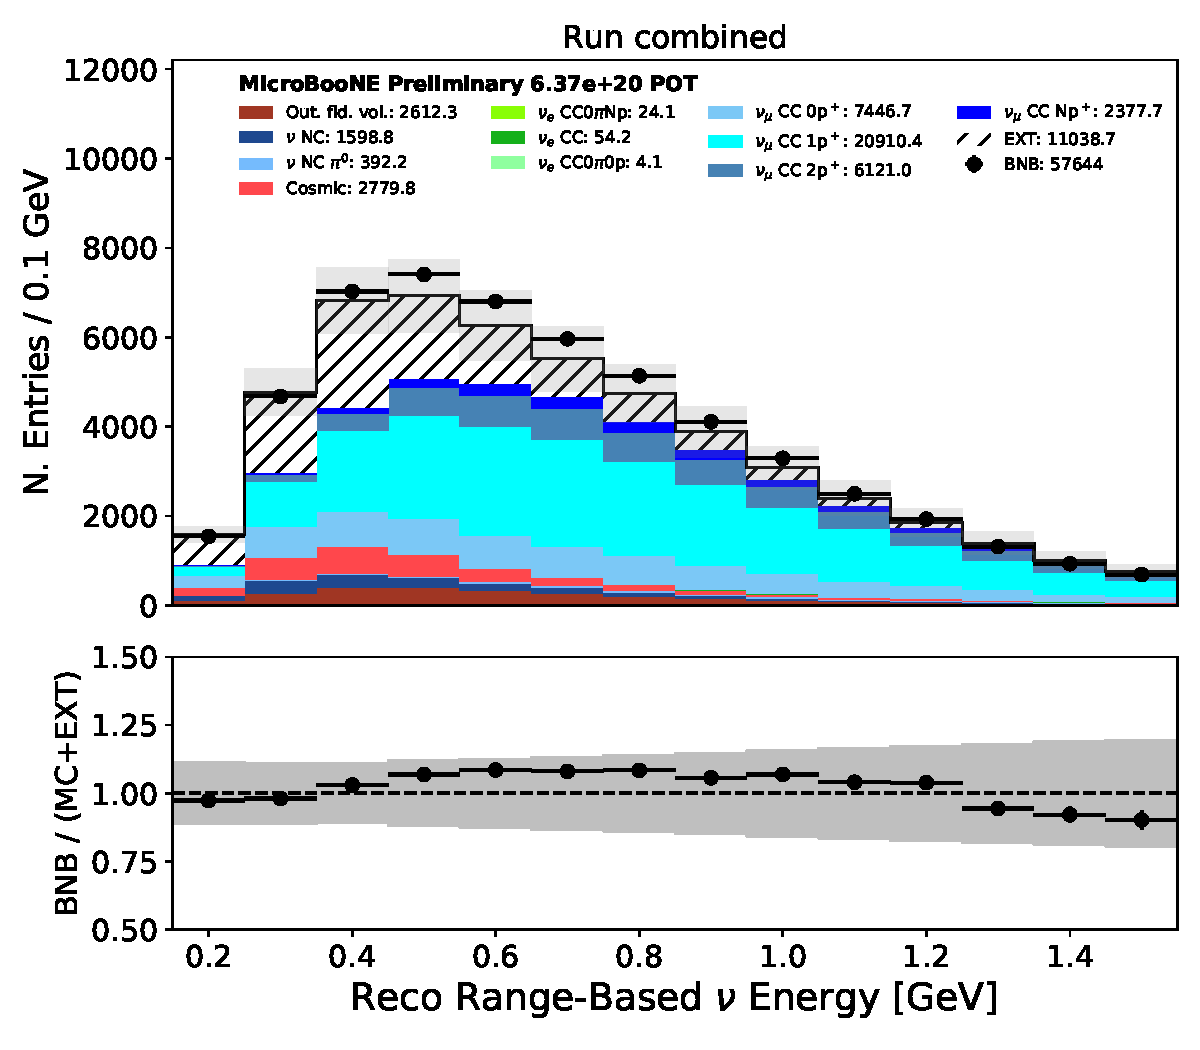
\includegraphics[width=1.00\textwidth]{NuMuCCsel/Images/Ryan/combined/reco_nu_e_range_v_08052020_full_samples_longest_noCRT_event_category.pdf}
    \caption{\label{fig:NuMUCCsel:ryan:combinedkinematics:nuE}}
    \end{subfigure}
    \begin{subfigure}[b]{0.3\textwidth}
    \centering
    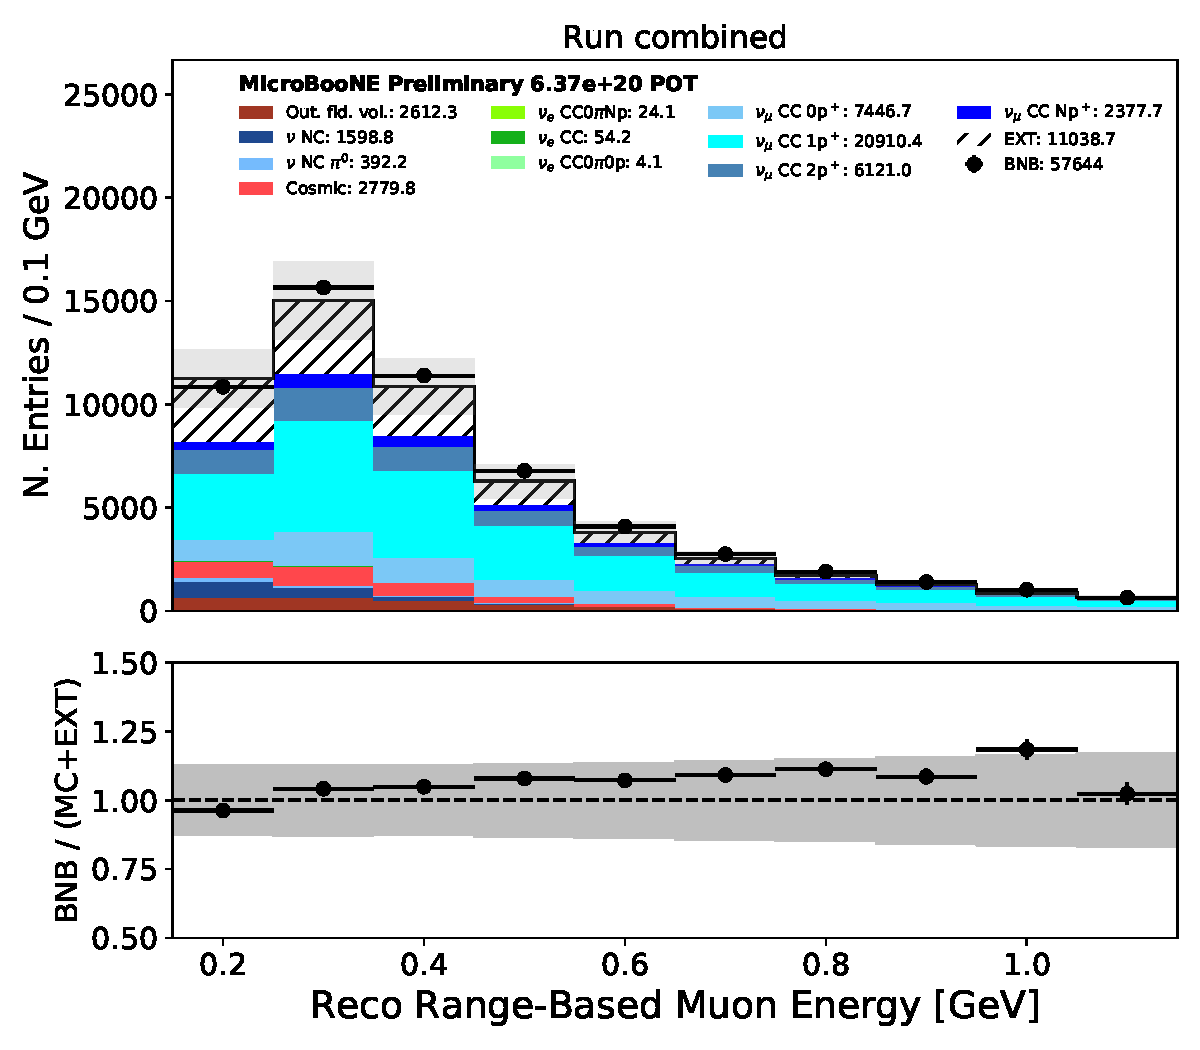
\includegraphics[width=1.00\textwidth]{NuMuCCsel/Images/Ryan/combined/trk_range_muon_e_v_08052020_full_samples_longest_noCRT_event_category.pdf}
    \caption{\label{fig:NuMUCCsel:ryan:combinedkinematics:muonE}}
    \end{subfigure} %\newline
    \begin{subfigure}[b]{0.3\textwidth}
    \centering
    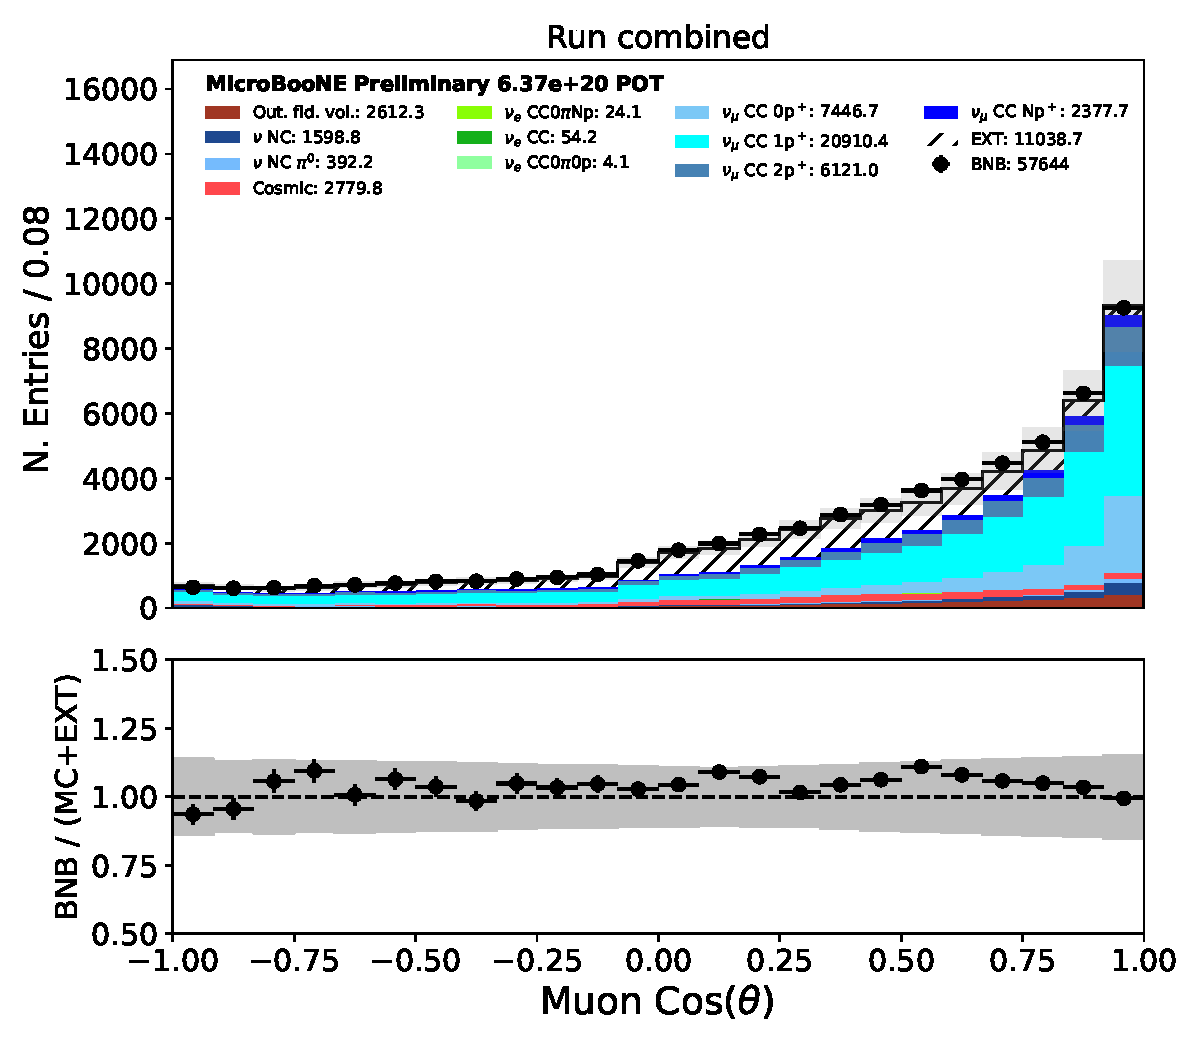
\includegraphics[width=1.00\textwidth]{NuMuCCsel/Images/Ryan/combined/trk_cos_theta_v_08052020_full_samples_longest_noCRT_event_category.pdf}
    \caption{\label{fig:NuMUCCsel:ryan:combinedkinematics:costheta}}
    \end{subfigure}
\caption{Distributions from the full $\nu_{\mu}$ CC INC selection with the $6.37e20$ POT of open data from Runs 1, 2, and 3 combined. MC systematic errors are included, with statistical errors, in MC error calculation.}
\label{fig:NuMuCCsel:ryan:runscombinedkinematics}
\end{center}
\end{figure}


%---------------------TIME DEPENDENCE-------------------------%
\subsection{Time Dependence}
\label{ssec:NuMUCCsel:timedep}
\par Run 3 is the only run considered when applying the $\nu_{\mu}$ constraint, as it is the only run where the CRT cuts are available. This method is only appropriate if Run 3 is a good proxy for the data as a whole. This time dependence study demonstrates the uniformity of run 3 in the context of all the open MicroBooNE data as a whole.

\par Because the CRT cuts cannot be applied to all runs, they will be applied to none of the distributions of this section; this direct comparison is more appropriate for this study as well. MC systematic errors (flux, GENIE, and G4) as well as statistics errors are included in all distributions. The main take-away from all of these plots should be that the data and Monte Carlo agree to within the error for virtually every distribution; in the individual runs as well as combined. Hints of DATA-MC disagreement in certain plots are quenched by the combined POT distributions.

\par Most of the plots for the time dependence study are in the appendix, section \ref{ssec:Appendix:numu:timedep}; with the exception of the reconstructed neutrino energy, fig \ref{fig:NuMuCCsel:timedep:Enu}, in this section. The plots displayed in the appendix are chosen to demonstrate the time dependence at various stages of the selection: SliceID filter only, preselection, and full selection. The data-MC agrees within the plotted errors (just detector systematic errors not included), with minor exceptions. For example, with the X coordinate of the reconstructed neutrino vertex, fig \ref{fig:NuMuCCsel:timedep:vtxX}, the run 3 distribution has disagreement at high and low x. This disagreement is only evident in this variable before any selection cuts are applied; fig \ref{fig:systematics:run3:nuvtxx} shows the same distribution but with the preselection applied (including CRT cuts) and the data agrees with MC to within the errors here. In fig \ref{fig:NuMuCCsel:timedep:vtxX_fullsel}, with the full selection applied but not CRT cuts, one can see that the disagreement is still within error bars. The CRT cuts should further reduce the disagreement near the edges of the distribution.

\par If one tries to add up the event counts of each category for the individual runs, they will find that they will not recover the value shown for the combined runs. This is most likely due to the normalization procedure used here. Each run is scaled with a flat POT normalization in addition to a finer tuning that comes from the GENIE simulation. The flat scaling factor averages over whatever intra-run effects might exist, introducing some rounding errors.

\par Each Run represents a year's worth of data taking, so intra-run effects should be considered. The run numbers are consecutive in time, each run lasting on the order of hours, so plotting out the data and MC as a function of run number roughly shows the chronology of data-taking, see \cref{fig:NuMuCCsel:timedep:RunsDistribution}. The white, hashed component of the histogram represents the OFF BEAM, or EXT, data. The OFF BEAM sample was collected almost entirely \textit{after} the ON BEAM data for Runs 1 and 2, but not Run 3. In order to probe the time dependence of the OFF BEAM sample, one can examine the distributions of variables that isolate the cosmic muon contribution in various stages of the selection. The topological score, seen in \cref{fig:NuMuCCsel:timedep:topo} and Cos($\theta$), fig \ref{fig:NuMuCCsel:timedep:costheta}, are such variables. There does not seem to be any time dependence with the shape of the EXT (OFF BEAM) component. The right-most bin of the topological score seems to be developing a deficit, but this could be due to statistics also the combined distribution agrees quite well for this bin.

\begin{figure}[hbt!] 
\begin{center}
    \begin{subfigure}[b]{0.35\textwidth}
        \centering
        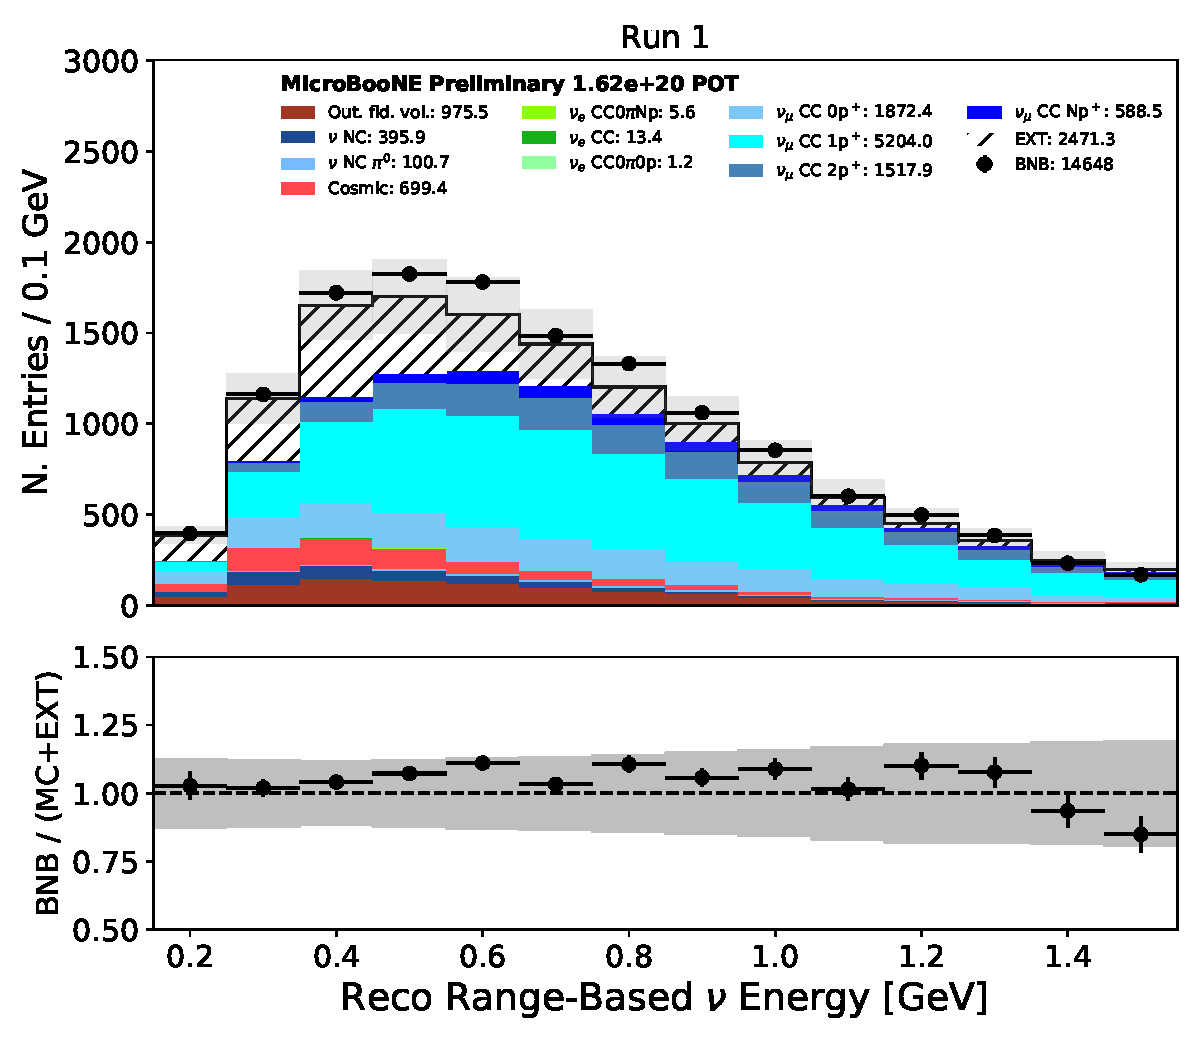
\includegraphics[width=1.00\textwidth]{NuMuCCsel/Images/Ryan/Run1/reco_nu_e_range_v_08052020_full_samples_longest_noCRT_event_category.pdf}
    \end{subfigure}
    \begin{subfigure}[b]{0.35\textwidth}
        \centering
        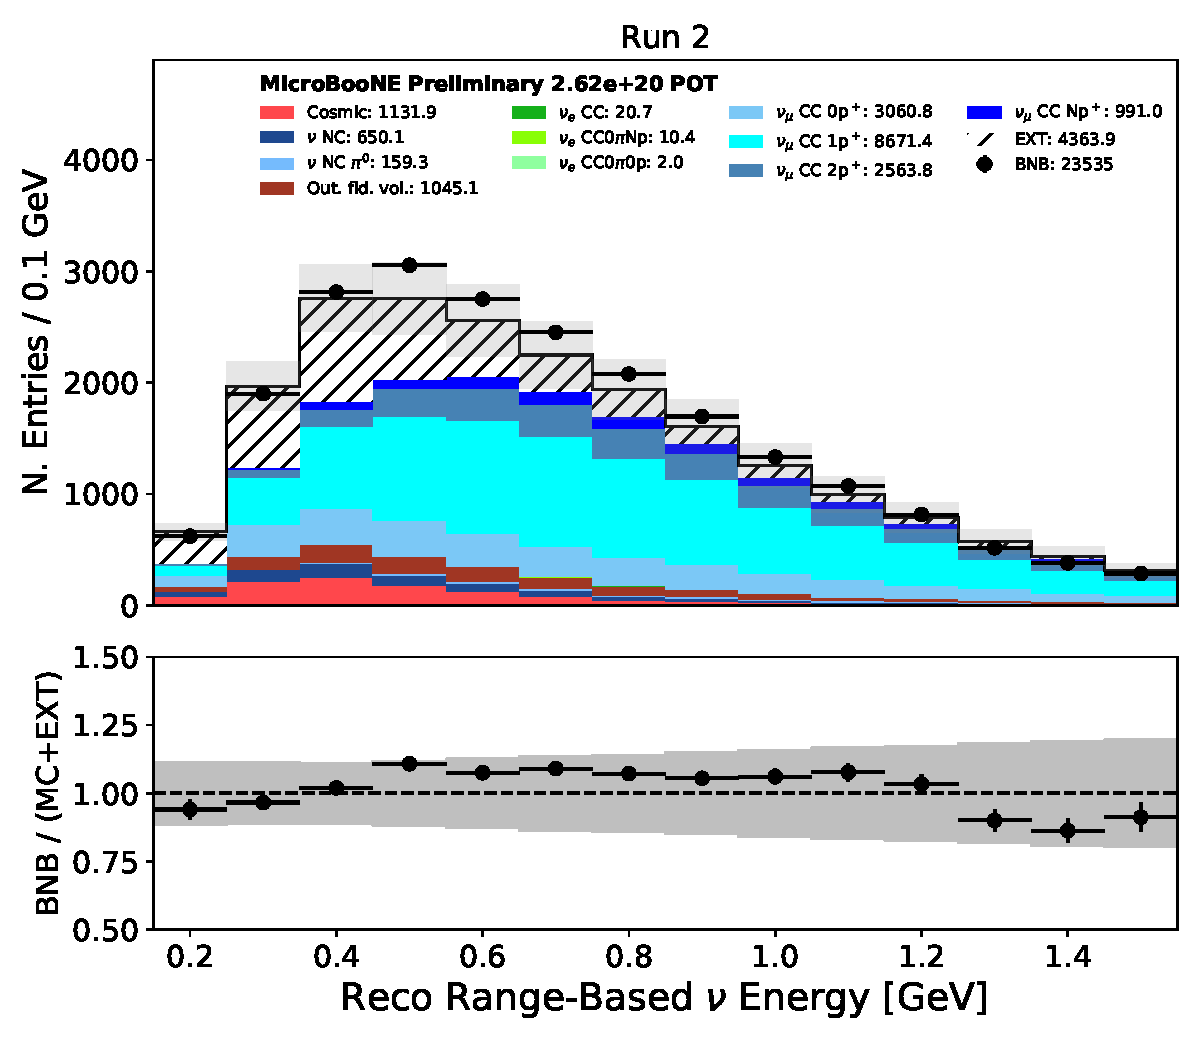
\includegraphics[width=1.00\textwidth]{NuMuCCsel/Images/Ryan/Run2/reco_nu_e_range_v_08052020_full_samples_longest_noCRT_event_category.pdf}
    \end{subfigure}
    \begin{subfigure}[b]{0.35\textwidth}
        \centering
        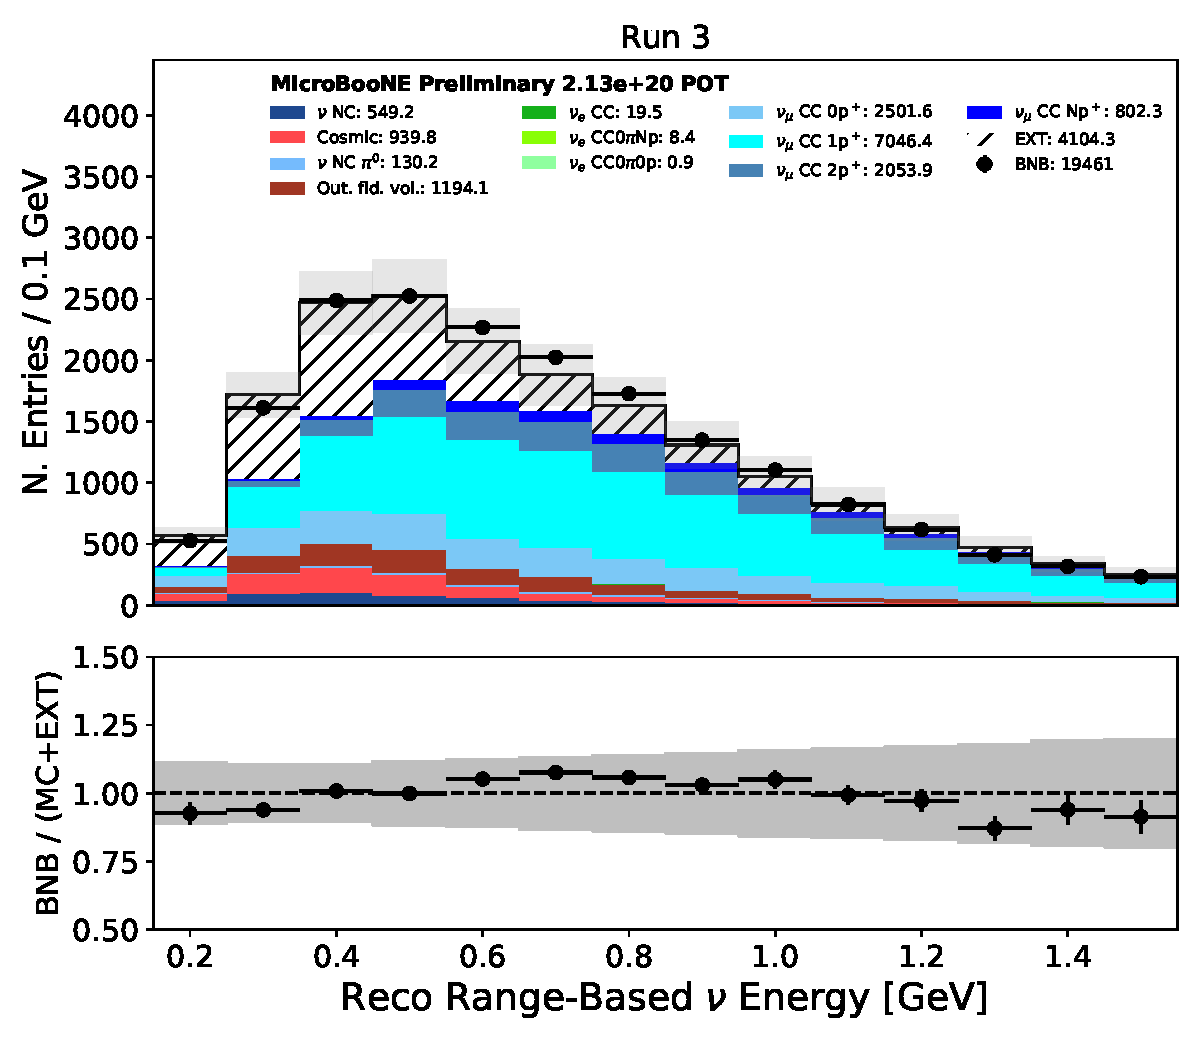
\includegraphics[width=1.00\textwidth]{NuMuCCsel/Images/Ryan/Run3_nocrt/reco_nu_e_range_v_08052020_full_samples_longest_noCRT_event_category.pdf}
    \end{subfigure} %\newline
    \begin{subfigure}[b]{0.35\textwidth}
        \centering
        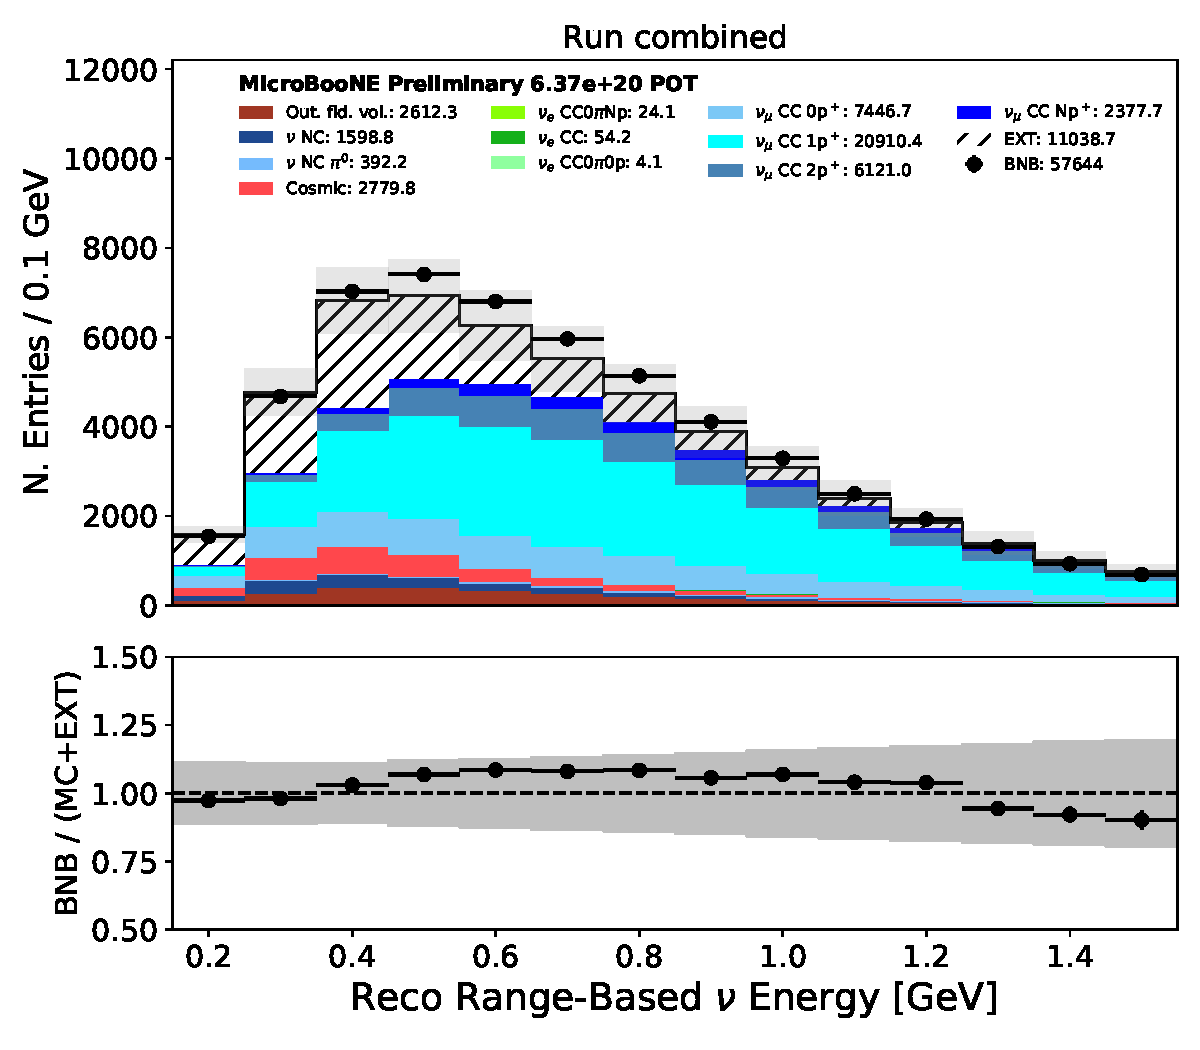
\includegraphics[width=1.00\textwidth]{NuMuCCsel/Images/Ryan/combined/reco_nu_e_range_v_08052020_full_samples_longest_noCRT_event_category.pdf}
    \end{subfigure}
\caption{Reconstructed neutrino energy for the open data sets of each run all open data combined.}
\label{fig:NuMuCCsel:timedep:Enu}
\end{center}
\end{figure}

\clearpage

